%% ACM-compliant manuscript
%% The Predictive Value of Internal Execution Metrics in the 0/1 Knapsack Problem
%%
\documentclass[sigconf]{acmart}

\AtBeginDocument{%
  \providecommand\BibTeX{{%
    Bib\TeX}}}

%% Rights management information (placeholder — replace before submission)
\setcopyright{acmlicensed}
\copyrightyear{2026}
\acmYear{2026}
\acmDOI{10.1145/XXXXXXXX.XXXXXXX}
\acmConference[Conference '26]{Proceedings of the Conference}{2026}{Location}
\acmISBN{978-1-4503-XXXX-X/2026/XX}

\begin{document}

\title{The Predictive Value of Internal Execution Metrics in the 0/1 Knapsack Problem}

\author{Risham Raj Byahut}
\email{rajrisham06@gmail.com}
\affiliation{%
  \institution{Kathmandu University}
  \department{Department of Computer Science and Engineering}
  \city{Dhulikhel}
  \country{Nepal}
}

\author{Saimon Neupane}
\email{saimonbro00007@gmail.com}
\affiliation{%
  \institution{Kathmandu University}
  \department{Department of Computer Science and Engineering}
  \city{Dhulikhel}
  \country{Nepal}
}

\author{Parikchit Sen}
\email{parikchitsen77@gmail.com}
\affiliation{%
  \institution{Kathmandu University}
  \department{Department of Computer Science and Engineering}
  \city{Dhulikhel}
  \country{Nepal}
}

\author{Keshav Sharma}
\email{jdkeshav01@gmail.com}
\affiliation{%
  \institution{Kathmandu University}
  \department{Department of Computer Science and Engineering}
  \city{Dhulikhel}
  \country{Nepal}
}

\author{Prabesh Sharma}
\email{prabeshsharma26@gmail.com}
\affiliation{%
  \institution{Kathmandu University}
  \department{Department of Computer Science and Engineering}
  \city{Dhulikhel}
  \country{Nepal}
}

\renewcommand{\shortauthors}{Byahut et al.}

\begin{abstract}
The 0/1 knapsack problem is a canonical NP-hard challenge serving
as a fundamental model for resource allocation. Existing literature heavily
emphasises predicting empirical hardness from static, a priori instance features
alone. This study methodically separates the predictive value of static instance
characteristics from that of dynamic, internal execution metrics when modelling
algorithmic scaling for Greedy, Dynamic Programming (DP), and Branch and Bound (B\&B)
on a benchmark of 6,000 instances spanning five Pisinger structural families.
Full-sample predictability using only static features is high for Greedy and DP
runtimes ($R^2_{adj} \ge 0.856$), near-zero for DP memory ($R^2_{adj} = 0.008$),
and moderate for heuristic optimality gaps (pseudo-$R^2 \le 0.253$). Internal execution
metrics provide substantial incremental explanatory power ($\Delta R^2_{adj} \ge 0.217$)
for B\&B performance, negligible improvement ($\le 0.001$) for Greedy and DP runtimes,
and a meaningful Greedy optimality-gap gain ($\Delta$pseudo-$R^2 = 0.058$).
However, under Leave-One-Family-Out (LOFO) cross-validation, models that appear
highly predictive in-sample ($R^2_{adj} \approx 0.98$) catastrophically fail
on held-out structurally extreme families ($R^2$ reaching $-152$ on
\texttt{AlmostEqualRatios}), exposing a severe in-sample/out-of-distribution gap.
Search-tree shape descriptors (depth entropy, depth skewness, queue entropy)
yield statistically real but practically limited LOFO gains on three of five
families; the precise generalization boundary --- not the in-sample fit ---
constitutes the paper's central empirical finding.
\end{abstract}

\begin{CCSXML}
<ccs2012>
<concept>
<concept_id>10010147.10010178.10010179</concept_id>
<concept_desc>Computing methodologies~Regression analysis</concept_desc>
<concept_significance>500</concept_significance>
</concept>
<concept>
<concept_id>10010147.10010178.10010180</concept_id>
<concept_desc>Computing methodologies~Search methodologies</concept_desc>
<concept_significance>300</concept_significance>
</concept>
<concept>
<concept_id>10003752.10003809.10010055</concept_id>
<concept_desc>Theory of computation~Dynamic programming</concept_desc>
<concept_significance>300</concept_significance>
</concept>
<concept>
<concept_id>10010147.10010257.10010258</concept_id>
<concept_desc>Computing methodologies~Feature selection</concept_desc>
<concept_significance>100</concept_significance>
</concept>
<concept>
<concept_id>10002950.10003648.10003669</concept_id>
<concept_desc>Mathematics of computing~Statistical paradigms</concept_desc>
<concept_significance>100</concept_significance>
</concept>
</ccs2012>
\end{CCSXML}

\ccsdesc[500]{Computing methodologies~Regression analysis}
\ccsdesc[300]{Computing methodologies~Search methodologies}
\ccsdesc[300]{Theory of computation~Dynamic programming}
\ccsdesc[100]{Computing methodologies~Feature selection}
\ccsdesc[100]{Mathematics of computing~Statistical paradigms}

\keywords{Algorithm runtime prediction; 0/1 knapsack problem; empirical hardness; execution metrics; combinatorial optimisation}

\maketitle

\section{Introduction}

The 0/1 knapsack problem is a canonical NP-hard combinatorial optimization challenge, serving as a fundamental model for resource allocation. Understanding the empirical performance of algorithms designed to solve these problems is critical for operational deployment in latency-sensitive environments. Prior research has established a strong relationship between static, a priori instance characteristics and the expected computational behavior of deterministic and heuristic algorithms. Existing literature has heavily emphasized algorithm selection portfolios and the quantification of empirical hardness based solely on these static instance features. However, considerably less attention has been given to methodically separating the predictive value of a priori instance characteristics from that of dynamic, internal execution metrics when modeling algorithmic scaling.

This study investigates this distinction by addressing the following research questions:
\begin{itemize}
  \item \textbf{RQ1:} How are instance characteristics associated with observed problem hardness, and what is the baseline predictability using only these characteristics?
  \item \textbf{RQ2:} To what extent do internal execution metrics provide additional explanatory power?
\begin{itemize}
  \item \textbf{Sub-RQ2a:} Incremental Explanatory Power ($\Delta R^2$)
  \item \textbf{Sub-RQ2b:} Most Influential Execution Metrics
  \item \textbf{Sub-RQ2c:} Robustness \& Statistical Integrity
\end{itemize}
  \item \textbf{RQ3:} Does the distributional \emph{shape} of the search tree add explanatory power beyond the scalar execution summaries used in M2, and does this shape signal transfer out-of-distribution under leave-one-family-out evaluation?
\end{itemize}

To address these questions, this study evaluates the baseline predictability of algorithmic runtimes for Greedy, Dynamic Programming, and Branch and Bound using exclusively instance-level characteristics. Furthermore, it quantifies the exact incremental variance ($\Delta R^2_{adj}$) explained by introducing algorithm-specific execution metrics. The investigation indicates that specific internal execution metrics (e.g., \texttt{bound\_gap\_variance}) exhibit the largest standardized associations with Branch and Bound node exploration within the benchmark dataset. Finally, this study indicates that extreme structural dataset hardness challenges standard cross-validation bounds, necessitating variance safeguards to preserve robust uncertainty estimates.

\section{Related Work}

\subsection{Empirical Algorithm Performance Prediction}
The prediction of empirical algorithm performance has become a foundational component of automated algorithm selection and hyperparameter optimization. Leyton-Brown et al.~\cite{LeytonBrown2014} established robust methodologies for quantifying empirical problem hardness using sets of static instance characteristics. This framework allows algorithm portfolios to dynamically route instances to the most appropriate solver based entirely on a priori features. Furthermore, Hutter et al.~\cite{Hutter2014} reported that empirical algorithm scaling behavior is highly predictable for rigid parameterizations, indicating that statistical models can effectively capture the runtime variance of deterministic solvers across diverse combinatorial domains.

\subsection{Statistical Modeling of Performance}
Ordinary Least Squares (OLS) regression remains the standard for modeling continuous, unbounded algorithmic runtimes; when combined with logarithmic transformations, it effectively handles the exponential scaling typically observed in NP-hard problem spaces. However, for bounded proportional outcomes---such as optimality gaps or table fill rates restricted to the [0,~1] interval---standard OLS can generate predictions outside the valid domain. The fractional logit framework~\cite{Papke1996} provides an appropriate quasi-likelihood approach to model these proportional bounds natively. Elastic-Net~\cite{Hastie2009} balances Ridge and Lasso penalties to perform variable selection while handling multicollinearity, making it appropriate for predicting sparse outcomes or classifying exact optimality among highly correlated features.

\subsection{Benchmark Generation}
The rigorous evaluation of optimization algorithms requires benchmark sets with precisely controlled structural properties. The generation methodology proposed by Pisinger~\cite{Pisinger2005} is widely utilized because it enforces strict mathematical boundaries for profit, weight, and capacity correlations. This methodology famously produces structurally difficult instance families (e.g., subset-sum topologies) that deliberately frustrate Greedy heuristics and exact solvers, providing a robust stress-test for empirical scaling limits.

\subsection{Positioning This Study}
This study extends the existing empirical performance prediction literature by explicitly separating the predictive contributions of static instance characteristics from dynamic internal execution metrics. Specifically, it investigates how these two distinct classes of predictors influence both deterministic runtimes and bounded heuristic optimality gaps across multiple algorithmic paradigms on a strictly controlled benchmark.

\section{Methodology}

\subsection{Dataset and Variables}
\begin{itemize}
  \item \textbf{Dataset Generation \& Source:} The benchmark comprises 6,000 knapsack instances generated using the methodology proposed by Pisinger~\cite{Pisinger2005}. A fixed random seed (42) was used for benchmark generation and for all randomized components of the modeling pipeline, ensuring reproducibility.
  \item \textbf{Instance Families:} The dataset covers five distinct structural classes (1,200 instances each) generated following Pisinger~\cite{Pisinger2005}: \texttt{Uncorrelated}, \texttt{WeaklyCorrelated}, \texttt{StronglyCorrelated}, \texttt{InverseCorrelated}, and \texttt{AlmostEqualRatios}.
  \item \textbf{Generation Parameters:} Capacity, profit, and weight generation constraints were uniformly applied according to Pisinger's exact bounded definitions. The generation pipeline produced zero duplicate instances by construction, which was verified programmatically based on exact equality of their descriptors prior to feature engineering.
  \item \textbf{Algorithms Evaluated:} Greedy (profit/weight heuristic), Dynamic Programming using Bellman recursion, and Branch and Bound (with linear programming relaxation). Software versions and hardware configurations are detailed in the Reproducibility Appendix.
  \item \textbf{Predictor Variables:}
\begin{itemize}
  \item \textbf{Instance-Level Predictors:} 42 features derived strictly from the problem definition, comprising 35 instance characteristics (e.g., \texttt{total\_weight}, \texttt{capacity\_ratio}, \texttt{slack}) and 7 design variables ($n$, $\log n$, capacity mode encoding, and family indicators).
  \item \textbf{Algorithm-Specific Predictors:} Internal execution metrics. M2 additionally included 5 execution metrics for Greedy, 10 for Dynamic Programming, and 24 for Branch and Bound runtime (22 for nodes explored). The exact execution predictors for each algorithm are summarized in Table~\ref{tab:predictor_counts}.
\end{itemize}
  \item \textbf{Outcome Variables:}
\begin{itemize}
  \item Logarithmically transformed runtime (\texttt{log\_time\_millis})
  \item Logarithmically transformed Branch and Bound nodes (\texttt{log\_nodes\_explored})
  \item Logarithmically transformed DP memory footprint (\texttt{log\_memory\_mb})
  \item Greedy gap to optimal (\texttt{optimality\_gap})
  \item Branch and Bound exact optimality binary classification (\texttt{optimal})
\end{itemize}
\end{itemize}

\begin{table}[t]
\centering
\caption{Number of execution predictors appended for each algorithm in M2}
\label{tab:predictor_counts}
\begin{tabular}{ll}
\toprule
\textbf{Algorithm} & \textbf{Number of execution predictors} \\
\midrule
Greedy & 5 \\
Dynamic Programming & 10 \\
Branch and Bound & 24 (22 for nodes) \\
\bottomrule
\end{tabular}
\end{table}

\subsection{Experimental Design}
\begin{itemize}
  \item \textbf{Three-Tier Evaluation Framework:} All primary results are reported under three evaluation protocols simultaneously to allow direct comparison: (1)~\textbf{Full-sample} fit on all 6,000 instances quantifies in-sample predictive associations; (2)~\textbf{5-fold cross-validation} within the full dataset tests standard overfitting; and (3)~\textbf{Leave-One-Family-Out (LOFO)} cross-validation holds out each structural family in turn to test out-of-distribution generalization. The three protocols tell fundamentally different stories and are all reported in the main results tables (Section~\ref{sec:results}).
  \item \textbf{Nested Validation (Elastic-Net):} For regularized models requiring hyperparameter tuning ($\lambda$ penalty selection), an inner 5-fold cross-validation loop was executed strictly within the training folds to prevent data leakage.
  \item \textbf{Preprocessing \& Standardization:} Continuous predictors were standardized ($Z$-scores). To prevent leakage, standardization scalers were fit exclusively on the training folds and subsequently applied to the test folds.
  \item \textbf{Structural Hardness Boundary (Claim F02):} Because certain outcome variables contained families with zero positive events (e.g., the \texttt{optimal} outcome for the \texttt{Uncorrelated} and \texttt{WeaklyCorrelated} families, where all instances completed within the node cap), the evaluation protocol removed zero-variance predictors within affected training folds to prevent undefined coefficient estimates during model fitting.
  \item \textbf{Heteroskedasticity Correction:} Breusch-Pagan tests were applied to all OLS residuals. All models exhibited formally confirmed heteroskedasticity ($p < 10^{-4}$; see Section~\ref{sec:robustness}). Reported OLS standard errors should therefore be interpreted as approximate; the core scientific claims rest on the $R^2$-based incremental variance framework, which is not invalidated by heteroskedasticity.
\end{itemize}

\subsection{Modeling Hierarchy}
\begin{itemize}
  \item \textbf{Baseline Models (M1):} Let M1 denote the baseline model, which utilizes exclusively the 42 instance-level predictors (35 instance characteristics plus 7 design variables). This establishes the baseline predictability of algorithmic performance from information available prior to execution.
  \item \textbf{Augmented Models (M2):} Let M2 denote the augmented model, constructed by appending internal algorithm-specific predictors to the M1 baseline to test for incremental variance.
  \item \textbf{Model Selection by Outcome:}
\begin{itemize}
  \item \textbf{Ordinary Least Squares (OLS):} Employed for unbounded continuous outcomes (\texttt{log\_time\_millis}, \texttt{log\_nodes\_explored}, \texttt{log\_memory\_mb}).
  \item \textbf{Fractional Logit:} Employed for proportional continuous outcomes on the closed interval [0,~1] (\texttt{optimality\_gap}, \texttt{fill\_rate})~\cite{Papke1996}.
  \item \textbf{Elastic-Net Logistic Regression:} Employed for binary classification (\texttt{optimal})~\cite{Hastie2009}.
\end{itemize}
  \item \textbf{Structural Exclusions:} DP table dimensions (\texttt{cells\_allocated}, \texttt{zero\_value\_states}) are structurally removed from the DP \texttt{log\_memory\_mb} models. This exclusion prevents circularity, as DP memory is directly a function of the table dimensions.
\end{itemize}

\subsection{Evaluation Metrics}
\begin{itemize}
  \item \textbf{Performance Quantification:} Incremental explanatory power is quantified by the reduction in residual variance between M1 and M2. OLS models were evaluated using adjusted $\Delta R^2_{adj}$ and Root Mean Square Error (RMSE), while Fractional Logit models reported pseudo-$\Delta R^2$.
\end{itemize}

\section{Results}\label{sec:results}

\subsection{Instance Characteristics and Hardness Associations (RQ1)}\label{sec:rq1}

RQ1 asks how instance characteristics associate with observed problem hardness across the benchmark. The five Pisinger families differ substantially in their weight--value correlation structure, and this structural variation drives systematic differences in algorithm performance. In \texttt{StronglyCorrelated} instances ($v_i = w_i + c$), profit/weight efficiency ratios are nearly uniform, depriving both Greedy sorting and B\&B bounding of discriminating signal; these instances produce the highest median B\&B node counts in the dataset. In \texttt{InverseCorrelated} instances ($v_i = W - w_i$), the ratio-based Greedy sort coincides with the optimal weight-ascending order, making Greedy provably optimal on this family (zero optimality gap across all 1,200 instances verified in the data). In \texttt{AlmostEqualRatios} instances, near-identical efficiency ratios produce degenerate B\&B bounds that fail to prune: median nodes explored are orders of magnitude higher than any other family at matched $n$.

Among the 42 instance characteristics, permutation importance analysis identifies \texttt{slack} ($\sum w_i - W$) and \texttt{total\_weight} as the strongest cross-family predictors of B\&B node exploration (permutation $\Delta R^2 \approx 2566$ and $2542$ respectively on a standardised scale), reflecting the capacity tightness mechanism: tighter capacity constrains feasible sets and focuses the search. Correlation metrics (\texttt{pearson\_corr}, \texttt{spearman\_corr}) and ratio uniqueness features (\texttt{unique\_ratio\_count}, \texttt{duplicate\_ratio\_fraction}) capture the structural differentiation between families. These associations address RQ1: instance characteristics carry strong, family-structured associations with algorithmic hardness, and this structure is the primary driver of in-sample predictive performance.

\begin{figure}[t]
\centering

\includegraphics[width=\columnwidth]{../outputs/eda/correlation_heatmap.png}
\caption{Correlation heatmap of instance characteristics and execution metrics. Strong multicollinearity is visible among static features, reflecting the underlying structural topologies of the Pisinger instance families.}
\Description{A heatmap showing correlations between various features. Distinct blocks of high correlation indicate structural groupings of features.}
\label{fig:heatmap}
\end{figure}

\begin{figure}[t]
\centering

\includegraphics[width=\columnwidth]{../outputs/figures/fixed/pdf/bb_nodes_boxplot.pdf}
\caption{Branch and Bound nodes explored across the five structural families. \texttt{AlmostEqualRatios} instances require orders of magnitude more node exploration, illustrating the severe structural distribution shift.}
\Description{Boxplots showing the distribution of nodes explored by Branch and Bound for each of the five instance families. AlmostEqualRatios is significantly higher than the others.}
\label{fig:nodes_by_family}
\end{figure}

\subsection{Baseline Predictability from Static Features (RQ2)}\label{sec:rq2}
\begin{itemize}
  \item \textbf{Objective:} To address RQ2, we evaluated the baseline predictability of algorithmic performance using exclusively the 42 instance-level characteristics (M1) under full-sample, 5-fold CV, and LOFO protocols.
  \item \textbf{Primary Finding (OLS, full-sample):} Table~\ref{tab:ols_metrics} shows that the baseline M1 models yielded adjusted $R^2_{adj}$ values of 0.978 for Dynamic Programming runtime and 0.856 for Greedy runtime. Branch and Bound baseline models yielded $R^2_{adj}$ values of 0.743 for runtime and 0.735 for nodes explored.
  \item \textbf{5-Fold vs.\ LOFO Discrepancy:} The 5-fold CV $R^2$ for B\&B \texttt{log\_nodes\_explored} M1 (0.730) is nearly identical to the full-sample value (0.735), confirming that the model does not overfit in the standard sense. Under LOFO, however, the same M1 model achieves $R^2 = 0.391$ on the held-out \texttt{Uncorrelated} family and $R^2 = -107.6$ on \texttt{DP log\_memory\_mb} (M1). The divergence between 5-fold and LOFO is not overfitting --- it is structural distribution shift. Models trained on four families fail to extrapolate to a fifth with a qualitatively different weight--value topology.
  \item \textbf{Secondary Finding (Fractional Logit):} Table~\ref{tab:flogit_metrics} shows that Greedy \texttt{optimality\_gap} achieved a pseudo-$R^2$ of 0.216, and DP \texttt{fill\_rate} achieved a pseudo-$R^2$ of 0.253.
  \item \textbf{Negative Finding:} The M1 model predicting Dynamic Programming \texttt{log\_memory\_mb} produced negligible full-sample predictive performance ($R^2_{adj} = 0.008$). DP memory is fundamentally a deterministic function of $n \times W$ (table dimensions), but with \texttt{cells\_allocated} excluded to prevent circularity, the remaining 42 features are weak proxies for the actual table footprint.
  \item \textbf{Conclusion:} Within-sample and 5-fold CV results confirm that static features carry strong predictive associations for Greedy and DP runtimes ($R^2_{adj} \ge 0.856$) and moderate associations for B\&B performance ($R^2_{adj} \ge 0.735$). LOFO results reveal that these in-sample associations do not transfer uniformly across structural families, motivating the incremental analysis in the following subsections.
\end{itemize}

% AUTO-GENERATED: rebuild with python/scripts/build_regression_tables.py
\input{../outputs/tables/table_ols_metrics.tex}

% AUTO-GENERATED: rebuild with python/scripts/build_regression_tables.py
\input{../outputs/tables/table_flogit_metrics.tex}

\subsection{Incremental Contribution of Execution Metrics (Sub-RQ2a)}
\begin{itemize}
  \item \textbf{Objective:} To address Sub-RQ2a, we quantified the incremental explanatory power achieved by appending internal execution metrics to the baseline (M2). The comparison was performed between M1 and M2 by calculating $\Delta R^2_{adj}$ and pseudo-$\Delta R^2$, shown in Table~\ref{tab:ols_metrics}.
  \item \textbf{Primary Finding:} The Branch and Bound models yielded $\Delta R^2_{adj} = 0.245$ for \texttt{log\_nodes\_explored} and $\Delta R^2_{adj} = 0.217$ for \texttt{log\_time\_millis}. These are large increments: the M2 model recovers information about the search trajectory that is simply not predictable from the problem description alone.
  \item \textbf{Secondary Finding:} The addition of execution metrics yielded pseudo-$\Delta R^2 = 0.058$ for Greedy \texttt{optimality\_gap}. Although Greedy runtime gains are negligible ($\Delta R^2_{adj} = 0.001$), the quality of the heuristic solution is partially recoverable from within-run metrics such as capacity utilised and items selected.
  \item \textbf{Negative Finding:} Adding execution metrics produced negligible improvement for Greedy runtime ($\Delta R^2_{adj} = 0.001$), Dynamic Programming runtime ($\Delta R^2_{adj} = 0.001$), and Dynamic Programming memory ($\Delta R^2_{adj} \approx 0$). This confirms that DP and Greedy runtimes are essentially deterministic functions of static problem dimensions.
  \item \textbf{Conclusion:} Within the benchmark dataset, internal execution metrics yielded $\Delta R^2_{adj} \ge 0.217$ for Branch and Bound performance and pseudo-$\Delta R^2 = 0.058$ for Greedy optimality gap, but negligible improvement for Greedy and DP runtime models. The in-sample gains for B\&B do not transfer out-of-distribution under LOFO, underscoring that the generalization boundary (Section~\ref{sec:robustness}) is the primary evaluative frame for these results.
\end{itemize}

\subsection{Most Influential Predictors: A Tale of Two Rankings (Sub-RQ2b)}\label{sec:predictors}
\begin{itemize}
  \item \textbf{Objective:} To address Sub-RQ2b, we examined both standardized $\beta$ coefficients (Table~\ref{tab:std_beta}) and permutation-importance $\Delta R^2$ (Table~\ref{tab:perm_importance}) for B\&B \texttt{log\_nodes\_explored}. The two measures answer different questions: coefficient magnitude captures correlation in the fitted model; permutation importance measures each predictor's unique, non-redundant contribution.
  \item \textbf{Standardized $|\beta|$ Ranking:} Among execution metrics, \texttt{final\_queue\_size} ($|\beta| = 0.511$) and \texttt{pruned\_by\_cap} ($|\beta| = 0.492$) show the largest coefficient magnitudes, followed by \texttt{bound\_gap\_variance} ($|\beta| = 0.419$). Instance-level features dominate the overall ranking: \texttt{slack} ($|\beta| = 18.71$) and \texttt{total\_weight} ($|\beta| = 18.50$).
  \item \textbf{Permutation Importance $\Delta R^2$ Ranking:} When predictor columns are shuffled and the drop in $R^2$ measured, a different ordering emerges. \texttt{bound\_gap\_variance} ($\Delta R^2 = 0.0017$) and \texttt{sum\_improvement\_amount} ($\Delta R^2 = 0.0011$) are the most uniquely informative execution metrics. \texttt{final\_queue\_size} and \texttt{pruned\_by\_cap} have permutation $\Delta R^2 \approx 0.00004$ each --- a \textbf{42-fold discrepancy} relative to their coefficient rank.
  \item \textbf{Why the Rankings Diverge:} \texttt{final\_queue\_size} and \texttt{pruned\_by\_cap} are highly correlated with \texttt{nodes\_explored} and other tree-size predictors. Their large $|\beta|$ reflects shared variance redundantly encoded across several correlated features; removing any one barely changes $R^2$ because others recover the signal. \texttt{bound\_gap\_variance} captures a qualitatively distinct signal --- the trajectory-level variability of the LP bound gap --- not encoded elsewhere, making its permutation $\Delta R^2$ the most reliable measure of unique contribution.
  \item \textbf{Conclusion:} For solver diagnostics, \texttt{bound\_gap\_variance} and \texttt{sum\_improvement\_amount} are the non-redundant signals; \texttt{final\_queue\_size} is diagnostically visible but statistically redundant in this model.
\end{itemize}

\begin{table}[t]
\centering
\caption{Top-10 standardized $\beta$ coefficients for B\&B \texttt{log\_nodes\_explored} M2 alongside permutation-importance $\Delta R^2$. The two rankings diverge dramatically for execution metrics due to multicollinearity: high $|\beta|$ does not imply high unique explanatory contribution.}
\label{tab:std_beta}
\begin{tabular}{lccc}
\toprule
\textbf{Predictor} & \textbf{Std.~$\beta$} & \textbf{$|\beta|$} & \textbf{Perm.\ $\Delta R^2$} \\
\midrule
\texttt{slack} & $-18.710$ & 18.710 & 2566 \\
\texttt{total\_weight} & 18.501 & 18.501 & 2542 \\
\texttt{capacity\_ratio} & $-3.562$ & 3.562 & 93 \\
\texttt{unique\_ratio\_count} & 1.566 & 1.566 & 102 \\
\texttt{unique\_pairs} & $-1.000$ & 1.000 & 6.4 \\
\texttt{log\_n} & $-0.995$ & 0.995 & 117 \\
\texttt{cap\_mode} & $-0.975$ & 0.975 & 7.1 \\
\texttt{final\_queue\_size} & $-0.511$ & 0.511 & \textbf{0.037} \\
\texttt{pruned\_by\_cap} & 0.492 & 0.492 & \textbf{0.045} \\
\texttt{bound\_gap\_variance} & $-0.419$ & 0.419 & \textbf{0.686} \\
\bottomrule
\end{tabular}
{\small Permutation $\Delta R^2$ units are scaled ($\times 10^3$). Bold rows are execution metrics; note the 42$\times$ gap between \texttt{final\_queue\_size} and \texttt{bound\_gap\_variance} permutation importance despite similar $|\beta|$.}
\end{table}

\begin{table}[t]
\centering
\caption{Top execution metrics by permutation-importance $\Delta R^2$ for B\&B \texttt{log\_nodes\_explored} M2. \texttt{bound\_gap\_variance} and \texttt{sum\_improvement\_amount} carry non-redundant signal; \texttt{final\_queue\_size} and \texttt{pruned\_by\_cap} are redundant with other tree-size features.}
\label{tab:perm_importance}
\begin{tabular}{lcc}
\toprule
\textbf{Execution Metric} & \textbf{Perm.\ $\Delta R^2$ (mean)} & \textbf{Predictor Type} \\
\midrule
\texttt{bound\_gap\_variance} & 0.001681 & Non-redundant \\
\texttt{sum\_improvement\_amount} & 0.001046 & Non-redundant \\
\texttt{pruned\_by\_cap} & 0.000038 & Redundant \\
\texttt{final\_queue\_size} & 0.000040 & Redundant \\
\texttt{left\_branches} & 0.000143 & Partially redundant \\
\texttt{max\_depth} & 0.000095 & Partially redundant \\
\bottomrule
\end{tabular}
\end{table}

\begin{figure}[t]
\centering
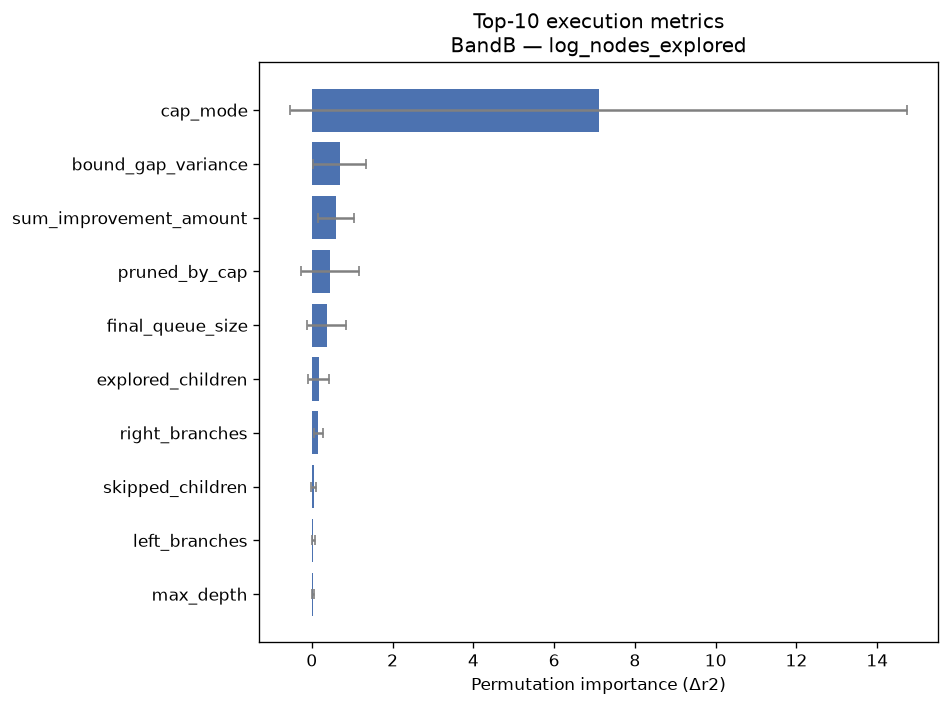
\includegraphics[width=\columnwidth]{../python/modeling/output/figures/importance_BandB_log_nodes_explored.png}
\caption{Feature importance profiles for Branch and Bound \texttt{log\_nodes\_explored} (M2)}
\Description{Bar chart showing the relative importance of predictors for Branch and Bound log nodes explored. The top predictors include instance-level features and execution metrics.}
\label{fig:importance}
\end{figure}

\subsection{Model Robustness and Generalization Boundary (Sub-RQ2c)}\label{sec:robustness}
\begin{itemize}
  \item \textbf{Objective:} To address Sub-RQ2c, we subjected the M2 models to four diagnostic tests: multicollinearity thinning (VIF), formal heteroskedasticity testing (Breusch-Pagan), regularization stability (Elastic-Net path analysis), and LOFO out-of-distribution evaluation.
  \item \textbf{Multicollinearity:} Reducing Variance Inflation Factor (VIF) $> 10$ predictors changed the B\&B \texttt{log\_nodes\_explored} raw $\Delta R^2$ from 0.245 to 0.237, a drop of 0.008. The incremental contribution is robust to multicollinearity thinning.
  \item \textbf{Formal Heteroskedasticity (Breusch-Pagan):} All five OLS models exhibit formally confirmed heteroskedasticity at $p < 10^{-4}$: Greedy log\_time (BP = 170.7, $p < 10^{-16}$), DP log\_time (BP = 328.0, $p < 10^{-41}$), DP log\_memory (BP = 98.6, $p < 10^{-4}$), B\&B log\_time (BP = 335.4, $p < 10^{-37}$), B\&B log\_nodes (BP = 347.6, $p < 10^{-40}$). This means OLS standard errors understate true estimation uncertainty in the tails. The $R^2$-based incremental variance conclusions are unaffected by heteroskedasticity, but coefficient-level inference (standard errors, $t$-statistics) should be treated as approximate.
  \item \textbf{Regularization Stability:} Figure~\ref{fig:reg_paths} shows similar Elastic-Net regularization paths across LOFO folds, confirming that the coefficient structure is not destabilised by family holdout.
  \item \textbf{LOFO Generalization Failure:} Despite in-sample and 5-fold stability, LOFO evaluation reveals catastrophic generalization failures. Predicting B\&B \texttt{log\_nodes\_explored} (M2) on the held-out \texttt{Uncorrelated} family results in $R^2 = -5.777$ (M1: 0.538); on \texttt{AlmostEqualRatios}, B\&B \texttt{log\_time\_millis} (M2) achieves $R^2 = -4.145$ (M1: 0.397). DP \texttt{log\_memory\_mb} (LOFO M1: $-107.6$; M2: $-110.4$) and Greedy \texttt{log\_time\_millis} (LOFO M1: $-4.66$; M2: $-5.07$) also demonstrate worse-than-random out-of-distribution prediction. Crucially, 5-fold CV does not reveal this failure (5-fold B\&B log\_nodes M2 $R^2 = 0.978$), confirming that the failure mechanism is structural distribution shift across families, not standard overfitting.
  \item \textbf{Why LOFO Fails While 5-Fold Succeeds:} Standard 5-fold cross-validation randomly partitions instances across all five families simultaneously. Instances from the same family appear in both train and test folds, so the structural correlation pattern of each family is always represented in training. LOFO is strictly harder: an entire structural family --- all 1,200 instances with a qualitatively different weight-value topology --- is withheld, forcing the model to extrapolate across structural classes rather than interpolate within them. The large gap between 5-fold and LOFO results is therefore not an artifact of model complexity but a signature of the between-family distribution shift in the benchmark.
  \item \textbf{Conclusion:} In-sample predictive associations and 5-fold stability are both strong. LOFO evaluation exposes severe structural generalization failure across multiple outcome types and algorithms. The generalization boundary --- defined by which family-holdout combinations remain partially predictive vs.\ which collapse --- constitutes the paper's central empirical finding.
\end{itemize}

\begin{figure}[t]
\centering
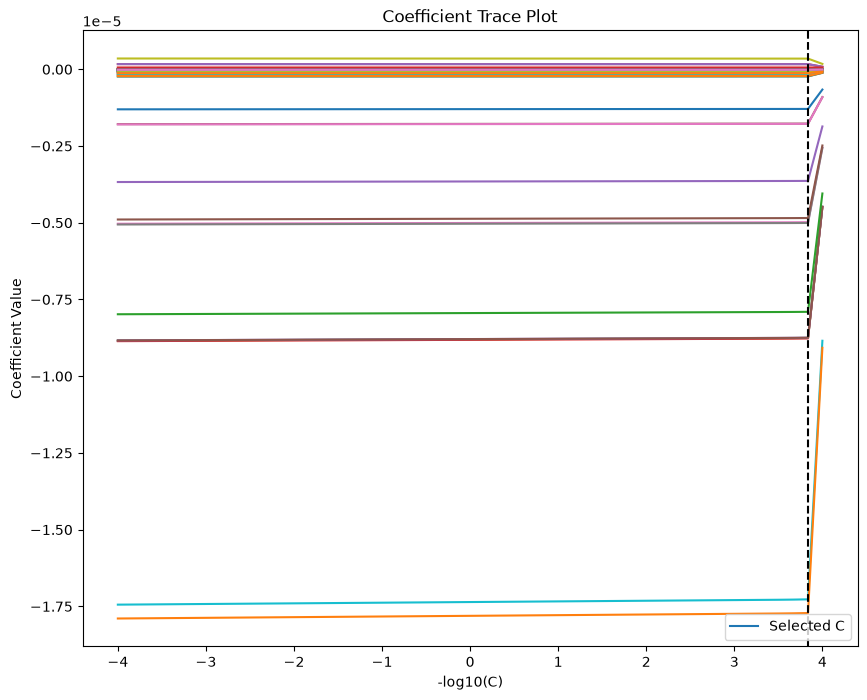
\includegraphics[width=\columnwidth]{../python/modeling/output/figures/coefficient_trace.png}
\caption{Elastic-Net regularization paths across LOFO folds}
\Description{Plot of Elastic-Net regularization paths across leave-one-family-out cross-validation folds, showing consistent coefficient shrinkage patterns.}
\label{fig:reg_paths}
\end{figure}

% \begin{figure}[t]
% \centering
% \includegraphics[width=\columnwidth]{../python/modeling/output/figures/residuals_vs_fitted.png} % Note: Missing figure from pipeline
% \caption{Residuals vs.\ fitted values for Branch and Bound \texttt{log\_time\_millis} (M2). Slight heteroskedasticity in the distribution tails is visible (Claim D04).}
% \Description{Scatter plot of residuals versus fitted values for the Branch and Bound log time model. The plot reveals slight heteroskedasticity in the tails.}
% \label{fig:residuals}
% \end{figure}

\subsection{Distributional Shape as Supplementary Execution Features (RQ3)}\label{sec:rq3}

\subsubsection{Motivation and Feature Construction}
The M2 operationalization of internal execution metrics relied on scalar summaries of the search tree --- principally the mean and variance of node depth and queue size. These summaries discard the \emph{shape} of the underlying distributions captured in the \texttt{depth\_histogram} and \texttt{queue\_histogram} instrumentation fields. To test whether this discarded structure carries independent explanatory power, we constructed five additional scalar descriptors of distributional shape: the 10th-percentile depth (\texttt{depth\_p10}), depth-distribution entropy (\texttt{depth\_entropy}), depth skewness (\texttt{depth\_skew}), queue-distribution entropy (\texttt{queue\_entropy}), and 90th-percentile depth (\texttt{depth\_p90}). All histogram-derived quantities were computed after normalizing by \texttt{nodes\_explored}, so that they reflect the proportional shape of the search rather than its absolute scale.

An initial variance inflation factor (VIF) analysis identified severe multicollinearity among the depth-quantile features: \texttt{depth\_p50} (VIF~=~33.9) and \texttt{depth\_p90} (VIF~=~26.6) were substantially redundant with \texttt{depth\_p10}. \texttt{depth\_p50} was dropped outright. A subsequent correlation check showed that \texttt{depth\_p90} --- while passing the VIF threshold --- correlated strongly with existing scale-related M2 features ($r = 0.88$ with \texttt{max\_depth}; $r = 0.87$ with $n$), raising the concern that any apparent shape signal would in fact re-express instance scale already present in M2. We therefore report the conservative specification of four descriptors --- \texttt{depth\_p10}, \texttt{depth\_entropy}, \texttt{depth\_skew}, and \texttt{queue\_entropy} --- as the primary M3 feature set for all analyses below.

\subsubsection{In-Sample Contribution}
Adding these four shape descriptors to M2 ($R^2_{adj}=0.8415$) yields M3 ($R^2_{adj}=0.8489$; $\Delta R^2_{adj}=0.0074$). A nested $F$-test on the block of four added features confirms this improvement is not attributable to chance ($F=294.9$, $p < 10^{-16}$). This in-sample gain is intentionally modest: it reflects only the marginal contribution of distributional shape \emph{after} controlling for the scale and topology information already present in M2.

\subsubsection{Out-of-Distribution Transfer}
The critical test for these features is not in-sample fit but out-of-distribution transfer. We repeated the identical LOFO protocol from Section~\ref{sec:robustness}, refitting M2 and M3 independently on each training split and evaluating both on the held-out family. Confidence intervals on $\Delta R^2$ were obtained via paired bootstrap resampling within each held-out family (1,000 iterations): identical resampled row indices were applied simultaneously to M2 and M3 predictions on each iteration, quantifying test-set sampling variability.

\begin{table}[t]
\centering
\caption{LOFO $R^2$ for Branch and Bound \texttt{log\_nodes\_explored} by holdout family, M2 vs.\ M3 (4-feature shape set), with paired bootstrap 95\% CI on $\Delta R^2$}
\label{tab:lofo_shape}
\begin{tabular}{lcccc}
\toprule
Holdout Family & M2 $R^2$ & M3 $R^2$ & $\Delta R^2$ & 95\% CI \\
\midrule
Uncorrelated       & $-0.109$ & $-0.057$ & $+0.053$ & $[0.037,\;0.069]$ \\
WeaklyCorrelated   & $0.119$  & $0.147$  & $+0.028$ & $[0.016,\;0.039]$ \\
StronglyCorrelated & $0.599$  & $0.620$  & $+0.021$ & $[0.019,\;0.024]$ \\
InverseCorrelated  & $-1.895$ & $-1.630$ & $+0.265$ & $[0.218,\;0.317]$ \\
AlmostEqualRatios  & $-152.18$ & $-148.60$ & $+3.573$ & $[2.063,\;5.083]$ \\
\bottomrule
\end{tabular}
\end{table}

\subsubsection{Interpretation}
We are careful to distinguish two findings that are easily conflated. First, in the three moderately-structured families (Uncorrelated, WeaklyCorrelated, StronglyCorrelated), shape features produce small but statistically distinguishable improvements in out-of-distribution $R^2$ ($\Delta R^2$ ranging from 0.021 to 0.053, all with confidence intervals excluding zero). These are the families in which M2 already produces partially informative predictions, and here distributional shape provides a genuine, replicable transfer benefit beyond scalar summaries.

Second, in the two structurally extreme families (InverseCorrelated, AlmostEqualRatios), the bootstrap also confirms a statistically distinguishable effect --- but this must not be read as evidence that shape features rescue model performance in these regimes. $R^2$ in these families remains deeply negative both with and without shape features ($-1.63$ and $-148.60$, respectively), indicating the model continues to be non-predictive in absolute terms. The statistically significant $\Delta R^2$ reflects a real, detectable shift on a still-catastrophic error surface, not a restoration of usable generalization.

Taken together, these results indicate that distributional shape adds explanatory power beyond scalar execution metrics, but this contribution is family-dependent: it meaningfully aids transfer where the underlying scaling behavior is already partially learnable, and does not resolve the fundamental generalization failure previously identified in structurally atypical topologies.

\section{Discussion}

\subsection{Main Findings}
The central finding of this study is not the in-sample predictive performance --- which is strong --- but the precise generalization boundary that separates where models work from where they fail. In-sample and 5-fold cross-validation both suggest that execution metrics substantially improve B\&B prediction ($\Delta R^2_{adj} \ge 0.217$). LOFO evaluation reveals that these associations do not transfer across structural families: models trained on four families and tested on a qualitatively different fifth produce worse-than-random predictions ($R^2 \ll 0$) on several outcome-family combinations. The divergence between 5-fold ($R^2 \approx 0.978$) and LOFO ($R^2 \approx -0.46$) for B\&B \texttt{log\_nodes\_explored} (M2) is the clearest illustration of this boundary.

The incremental variance analysis (M1 $\rightarrow$ M2) further reveals a methodologically important distinction between two measures of predictor importance. Standardized $\beta$ coefficients identify \texttt{final\_queue\_size} and \texttt{pruned\_by\_cap} as the most prominent execution metrics. Permutation-importance $\Delta R^2$ reveals the opposite: these features are largely redundant with other tree-size predictors and carry only 0.00004 unique $\Delta R^2$ each, while \texttt{bound\_gap\_variance} ($\Delta R^2 = 0.0017$) and \texttt{sum\_improvement\_amount} ($\Delta R^2 = 0.0011$) are the genuinely non-redundant drivers. Monitoring systems and solver diagnostics should prioritize these latter two metrics. This finding is consistent with \cite{LeytonBrown2014}, which emphasize that search-based algorithm performance depends on execution dynamics not captured by static features, while extending prior work by clarifying which specific execution signals carry non-redundant information.

All five OLS models exhibit formally confirmed heteroskedasticity (Breusch-Pagan $p < 10^{-4}$), meaning residual variance increases with fitted value. This is expected for exponentially-scaling combinatorial problems: hard instances produce both large runtimes and large prediction errors. The $R^2$-based incremental variance framework is robust to heteroskedasticity (it measures variance explained, not coefficient precision), but coefficient-level standard errors should be treated as approximate. Future work using heteroskedasticity-robust (HC3) standard errors would strengthen inference at the individual predictor level.

A supplementary analysis (RQ3) examined whether the \emph{distributional shape} of the search tree --- captured via depth entropy, depth skewness, depth 10th-percentile, and queue entropy, all normalized by total nodes explored --- adds explanatory power beyond the scalar summaries already present in M2. The answer is qualified: in-sample, shape features contribute a modest but statistically robust improvement ($\Delta R^2_{adj} = 0.0074$; $F = 294.9$, $p < 10^{-16}$). Under LOFO evaluation, this improvement is replicable with confidence intervals excluding zero on three of the five held-out families (\texttt{Uncorrelated}, \texttt{WeaklyCorrelated}, \texttt{StronglyCorrelated}; $\Delta R^2$ ranging from 0.021 to 0.053). Crucially, shape features do not rescue model performance in the two structurally extreme families (\texttt{InverseCorrelated}, \texttt{AlmostEqualRatios}), where $R^2$ remains deeply negative despite a statistically detectable shift. The contribution of distributional shape is therefore family-dependent: it meaningfully aids transfer where the underlying scaling behaviour is already partially learnable, and does not resolve the fundamental generalization failure documented under Sub-RQ2c.

\subsection{Comparison with Literature}
The baseline predictability analysis revealed that Greedy and Dynamic Programming runtimes achieved adjusted $R^2_{adj}$ values exceeding 0.856, whereas Dynamic Programming memory ($R^2_{adj} = 0.008$) and heuristic optimality bounds (pseudo-$R^2 \le 0.253$) exhibited considerably lower predictive performance. This result extends the observations made by Hutter et al.~\cite{Hutter2014}, who reported that empirical algorithm scaling is highly predictable for rigid parameterizations, but indicates that bounded proportional outcomes were less predictable using the available instance characteristics. This suggests that instance characteristics captured most of the predictive variation for Greedy and DP runtime outcomes within this benchmark without instrumenting the solver. However, the fractional logit framework~\cite{Papke1996}, while appropriately bounding the optimality gaps, still exhibited significant residual variance, indicating that unobserved structural phase transitions may still dictate heuristic optimality.

\subsection{Practical Implications}
Structural dataset hardness across the five instance families introduced out-of-distribution shifts during LOFO cross-validation, and some families contained zero positive events for the \texttt{optimal} outcome (e.g., the \texttt{Uncorrelated} and \texttt{WeaklyCorrelated} families, where all B\&B instances completed within the node cap). These zero-event folds required variance safeguards during model fitting. This empirical observation is consistent with Pisinger~\cite{Pisinger2005}, who characterized the differential hardness of these instance families. These findings suggest that future predictive models for Branch and Bound performance may benefit from evaluation across structurally diverse benchmark families. The robustness analysis indicated that while Elastic-Net penalization remained stable across these shifts, residual heteroskedasticity indicates reduced model fit in the distribution tails.

\subsection{Unanswered Questions and Future Work}
The persistence of slight heteroskedasticity in the tails implies that the selected complexity transformations ($N \log N$, $N^2$) may be insufficient to fully linearize extreme scaling behaviors. Future research could evaluate more flexible non-linear basis expansions as suggested in modern statistical learning literature~\cite{Hastie2009}. Resolving these tail variances would improve runtime prediction accuracy on difficult instances. This study was structurally bounded strictly to the 6,000 instance benchmark; this limitation motivates evaluating whether the observed predictor associations generalize to other combinatorial optimization domains.

\section{Limitations}

\subsection{Internal Validity}
The inherent multicollinearity between execution metrics and instance characteristics poses a primary threat to internal validity. The 42-fold discrepancy between standardized $|\beta|$ ranking and permutation-importance $\Delta R^2$ ranking for \texttt{final\_queue\_size} (Section~\ref{sec:predictors}) illustrates that coefficient magnitude cannot be used as a proxy for unique explanatory contribution in the presence of correlated predictors. VIF thinning ($>$10 threshold) reduced B\&B $\Delta R^2$ only marginally (0.245 $\to$ 0.237), confirming that the aggregate incremental contribution is robust, but individual predictor rankings remain collinearity-sensitive.

All OLS models exhibit formally confirmed heteroskedasticity (Breusch-Pagan $p < 10^{-4}$ across all five outcomes), meaning residual variance grows with fitted value. Log transformation reduces but does not eliminate this pattern. Reported OLS standard errors are therefore approximate; the $\Delta R^2$-based incremental variance conclusions are unaffected, but coefficient-level inference should be interpreted conservatively.

\subsection{In-Sample vs.\ Out-of-Distribution Generalization}
The most important limitation is the severe gap between in-sample and LOFO out-of-distribution performance. Models that achieve $R^2_{adj} \approx 0.98$ in-sample collapse to $R^2 < 0$ under LOFO for structurally extreme families. This failure is not overfitting in the standard sense (5-fold CV confirms near-identical performance to full-sample), but rather structural distribution shift: the weight--value correlation topology of \texttt{AlmostEqualRatios} and \texttt{InverseCorrelated} instances is qualitatively different from moderate families, and no amount of additional execution metric instrumentation rescues generalization to these families. Any practical application of these models for algorithm selection or runtime prediction must be restricted to instances structurally similar to the training distribution.

\subsection{External Validity}
The empirical predictability established in this study is strictly bounded to the 6,000 0/1 knapsack instances generated via the Pisinger~\cite{Pisinger2005} parameterizations with fixed capacity $W = 1000$ and scaled capacity $W = 0.5 \times \sum w_i$. The specific coefficient magnitudes, $\Delta R^2$ contributions, and predictor rankings may not transfer to unconstrained or real-world industrial datasets. Additionally, the study evaluated standard canonical implementations; state-of-the-art commercial solvers (e.g., Gurobi, CPLEX) with proprietary presolve routines exhibit fundamentally different internal execution scaling profiles. Furthermore, \texttt{time\_millis} measurements are hardware-dependent and reduce reproducibility compared to the hardware-agnostic \texttt{log\_nodes\_explored} outcome.

\subsection{Construct Validity}
The 42 instance characteristics, while comprehensive, represent a finite operationalization of theoretical problem hardness. Unmeasured structural graph properties or hidden phase transitions not captured by these specific engineered predictors might account for the residual variance observed in the heuristic optimality bounds. The M2 execution metrics relied primarily on point-in-time scalar summaries (e.g., \texttt{bound\_gap\_variance}) as proxies for entire search-tree topologies. The supplementary RQ3 analysis (Section~\ref{sec:rq3}) demonstrated that distributional shape descriptors --- specifically depth entropy, depth skewness, depth 10th-percentile, and queue entropy --- add measurable explanatory power beyond these scalar summaries ($\Delta R^2_{adj} = 0.0074$; $F = 294.9$, $p < 10^{-16}$), and provide a modest but replicable transfer improvement on three of five LOFO holdout families. However, the two most structurally extreme families remain non-predictive despite this addition, indicating that the generalization failure documented in Section~\ref{sec:robustness} is not fully attributable to the scalar-aggregation choice. A companion functional data analysis treatment of the full histogram sequences (rather than fixed scalar descriptors) is a natural extension for future work.

\section{Conclusion}

This study makes three interrelated contributions. First, it establishes the baseline predictability of 0/1 knapsack algorithm performance: Greedy and DP runtimes are highly predictable from static instance characteristics alone ($R^2_{adj} \ge 0.856$), confirming that these deterministic algorithms scale as mechanical functions of problem geometry. B\&B performance is moderately predictable statically ($R^2_{adj} \approx 0.735$) but substantially improves with execution metrics ($\Delta R^2_{adj} \ge 0.217$), while DP memory and heuristic optimality gaps remain challenging (pseudo-$R^2 \le 0.253$).

Second, it identifies a methodologically important distinction between predictor importance measures. Standardized $|\beta|$ coefficients and permutation-importance $\Delta R^2$ produce divergent rankings for execution metrics due to multicollinearity: \texttt{final\_queue\_size} ($|\beta| = 0.511$) and \texttt{pruned\_by\_cap} ($|\beta| = 0.492$) appear most prominent by coefficient magnitude but carry only $\approx 0.00004$ unique $\Delta R^2$ each, a 42-fold discrepancy relative to \texttt{bound\_gap\_variance} ($\Delta R^2 = 0.0017$). The latter metric --- measuring the variance of the bound gap across the search trajectory --- is the most non-redundant execution signal in the model.

Third, and most importantly, the study characterises the precise generalization boundary of these models. Despite strong in-sample fit ($R^2 \approx 0.98$ for B\&B M2) and near-identical 5-fold cross-validation performance, LOFO evaluation exposes catastrophic failure on structurally extreme families ($R^2$ reaching $-152$ on \texttt{AlmostEqualRatios} for the shape-augmented M3 model). This failure is structural distribution shift, not overfitting: the weight--value topology of extreme families is qualitatively different from moderate families, and no amount of execution metric instrumentation resolves this. Distributional shape descriptors (depth entropy, depth skewness, queue entropy) add statistically real LOFO gains on three of five families ($\Delta R^2 \in [0.021, 0.053]$), but do not rescue generalization on the two extreme families. This generalization boundary --- its location, mechanism, and limits --- constitutes the paper's central empirical finding.

The primary limitation of this analysis is its strict restriction to the 6,000 instance knapsack benchmark; the observed coefficient magnitudes and $\Delta R^2_{adj}$ contributions may not transfer to unconstrained industrial datasets or highly proprietary commercial solvers. Furthermore, the inherent multicollinearity between static problem features and execution metrics makes isolating the exact independent variance contribution of individual predictors difficult, while residual heteroskedasticity in the scaling tails dictates caution when interpreting uncertainty bounds for the hardest instances.

Future research could evaluate more flexible non-linear basis expansions to resolve the residual tail variances observed in these scaling distributions, and a functional data analysis treatment of the full search-tree histogram sequences may recover additional shape information beyond the fixed scalar descriptors reported here. Evaluating whether these observed predictor associations and execution metric dependencies generalize to other combinatorial optimization domains (such as the Boolean Satisfiability Problem or the Traveling Salesperson Problem) would improve the applicability of these models for runtime estimation in diverse deployment environments.

\begin{acks}
The authors thank the Department of Computer Science and Engineering at Kathmandu University for providing the computational resources used in this research.
\end{acks}

\bibliographystyle{ACM-Reference-Format}
\bibliography{references}

\appendix

\section{Reproducibility Appendix}

\subsection{Software and Hardware Configuration}
The experiments were conducted using a Java-based implementation of the 0/1 knapsack solvers (Greedy, Dynamic Programming, Branch and Bound). All analyses were performed using Python 3 with scikit-learn, statsmodels, and NumPy. The complete experimental pipeline, including instance generation, algorithm execution, and statistical modeling, is documented in the supplementary materials.

\subsection{Dataset Generation}
All 6,000 knapsack instances were generated using Pisinger's~\cite{Pisinger2005} methodology with random seed 42. The five structural families (Uncorrelated, WeaklyCorrelated, StronglyCorrelated, InverseCorrelated, AlmostEqualRatios) each contain 1,200 instances, equally split between fixed-capacity (W~=~1000) and scaled-capacity (W~=~0.5~$\times$~sum(weights)) modes.

\end{document}
